%%%%%%%%%%%%%%%%%%%%%%%%%%%%%%%%%%%%%%%%
% University/School Laboratory Report
% LaTeX Template
% Version 3.1 (25/3/14)
%
% This template has been downloaded from:
% http://www.LaTeXTemplates.com
%
% Original author:
% Linux and Unix Users Group at Virginia Tech Wiki 
% (https://vtluug.org/wiki/Example_LaTeX_chem_lab_report)
%
% License:
% CC BY-NC-SA 3.0 (http://creativecommons.org/licenses/by-nc-sa/3.0/)
%
%%%%%%%%%%%%%%%%%%%%%%%%%%%%%%%%%%%%%%%%%

%----------------------------------------------------------------------------------------
%   PACKAGES AND DOCUMENT CONFIGURATIONS
%----------------------------------------------------------------------------------------

\documentclass{article}

\usepackage[version=3]{mhchem} % Package for chemical equation typesetting
\usepackage{siunitx} % Provides the \SI{}{} and \si{} command for typesetting SI units
\usepackage{graphicx} % Required for the inclusion of images
\usepackage{natbib} % Required to change bibliography style to APA
\usepackage{amsmath} % Required for some math elements 
\usepackage{listings}
\usepackage{float}
\usepackage[center]{caption}
\usepackage{enumerate}
\usepackage{soul}
\usepackage{csquotes}
\usepackage{tcolorbox} 
\usepackage{minted}

%\setlength\parindent{0pt} % Removes all indentation from paragraphs

%\renewcommand{\labelenumi}{\alph{enumi}.} % Make numbering in the enumerate environment by letter rather than number (e.g. section 6)

%\usepackage{times} % Uncomment to use the Times New Roman font

%----------------------------------------------------------------------------------------
%   DOCUMENT INFORMATION
%----------------------------------------------------------------------------------------

\date{\today} % Date for the report

\begin{document}
% Define document title and author
\title{Fourier Methods}
\author{Johnny Pribyl}
\markboth{Montana State University}{}
\maketitle

\begin{abstract}

    This lab is designed to familiarize the student with thinking in the
    frequency domain. It requires far more data collection than the previous
    labs. There are four main objectives. First, we worked with a few simple
    input functions in order to become familiar with the spectrum analyzer.
    Second, we investigated the response of an LRC circuit to several different
    signal types. Third, we did the same thing to an acoustical cavity. And
    lastly, we examined a system of coupled torsional reed oscillators.
    Unfortunately, we ran out of time and were not able to collect all of the
    necessary data from the reed oscillators - so, this report will only
    include an informal discussion of theory and observed results.
    
\end{abstract}



%----------------------------------------------------------------------------------------
%   SECTION 1
%----------------------------------------------------------------------------------------
\section{Introduction}

Somehow, every undergraduate physics student manages to sneak through their
classes without ever fully understanding Fourier methods. Brian took it upon
himself to fill this educational hole with experimental knowledge. That means
this lab operates almost entirely in the frequency domain. Or, in other words,
we Fourier Transform \textit{everything}.

Although it's pretty tough to get funding these days, MSU still has some toys
leftover from the 90s. Among those is the SR770 Spectrum Analyzer. It boasts a
peaceful green-hued digital output and the capacity to live stream the
frequency domain of a time-dependent signal. It only lacks the phrase
\textit{\textbf{DON'T PANIC.}} Ideally, this would be inscribed in large
friendly letters on its cover.

We used the SR770 and TBS1052B-EDU oscilloscope extensively in this lab. Both
of them are capable of saving hundreds of data points at the press of a button.
So, we had quite a bit more real data to analyze for this lab than we have had
for any of our previous forays.

As before, you can find all of my code and data at:
\begin{verbatim}
    jpribyl/cautious-palm-tree
\end{verbatim}

\subsection{Database Design}%

The majority of this lab's data is relatively straightforward. Typically there
are two columns - one for the dependent variable (say, voltage) and one for the
independent variable (typically time or frequency). We saved this data into
.csv files on a USB. However, all of the measurements carry a large amount of
metadata regarding input frequency, amplitude, channel, and the source of the
data. Unfortunately, all of the metadata is not recorded into the files. We
wrote it all down in our lab notebooks, but that makes it difficult to cross
reference.

It would definitely be possible to store all the time / voltage data in excel
and assign values to the metadata with python as we read it in. However, that
approach does not scale very well. It's particularly ineffective for
collaborative efforts. Ideally, there would be a way to tie all of the
metadata to the files themselves. This ensures data integrity without
requiring all collaborators to use an identical code base. It turns out, I'm
not the first person in the world who has had this problem. The correct tool
for the job is a ``database." 

Databases are created and maintained with a language called SQL, or Structured
Query Language. Every measurement is given a unique identifier that allows
anyone to access or ``query" all of its metadata.

Our data did not come pre-packaged with unique identifiers, so I had to add
them manually. Bash has several incredibly powerful text-editing commands that
are perfect for this kind of task. I'm not as familiar with Awk, so I opted to
use Sed. If you have a bash shell on your computer you should be able to access
the man pages with 

\begin{verbatim}
    man sed
\end{verbatim}

Otherwise, you can read them online at gnu.org/software/sed/manual/sed.txt. The
first step was collecting all of our files into a single directory and naming
them numerically so that I can sort through them with a for loop:

\begin{figure}[thp]
\centering
\begin{minipage}{.8\textwidth}
\begin{tcolorbox}
\begin{minted}{bash}
    #!/bin/bash
    cur_id=1;

    for i in $(ls * | sort -V);
    do
        echo $i
        echo $cur_id

        #double quotes allow variables
        sed -i "s/\(.*\)/$cur_id,\1/" $i

        let cur_id+s=1
    done
\end{minted}
\end{tcolorbox}
\end{minipage}
\end{figure}

I find bash incredibly hard to read, so let's break this down a bit. The very
first line is known as a ``shebang" and tells the computer to use bash for this
script. Next I define a variable ``cur\_id" which holds the unique
identifier that will get prepended to every line of the data files.

After that I run through every file in the current directory and sort them
``naturally." For each file, I read out (or echo) the file name and the file's
identifier. Then, I tack the current id and a comma in front of every line in
the file and increment the cur\_id by 1.

Let's say that the first file in a given directory looks like this:
\begin{figure}[thp]
\centering
\begin{minipage}{.8\textwidth}
\begin{tcolorbox}
\begin{minted}{python} 
    0.0000000e+000, -1.3732910e-001,
    6.2500000e+001,  9.4042969e+000,
    ...
    1.2500000e+002, -4.9438477e-002,
    1.8750000e+002, -7.1411133e-002,
    2.5000000e+002, -3.2958984e-002,
    3.1250000e+002, -3.2958984e-002,
\end{minted}
\end{tcolorbox}
\end{minipage}
\end{figure}

My script will turn it into something that looks like this:
\begin{figure}[thp]
\centering
\begin{minipage}{.8\textwidth}
\begin{tcolorbox}
\begin{minted}{python} 
    1,  0.0000000e+000, -1.3732910e-001,
    1,  6.2500000e+001,  9.4042969e+000,
    ...
    1,  1.2500000e+002, -4.9438477e-002,
    1,  1.8750000e+002, -7.1411133e-002,
    1,  2.5000000e+002, -3.2958984e-002,
    1,  3.1250000e+002, -3.2958984e-002,
\end{minted}
\end{tcolorbox}
\end{minipage}
\end{figure}

Where 1 is the unique identifier for this measurement. The second file in the
directory would look very similar except that it would be prepended with a 2
instead of a 1. 

After pre-processing the data, I read it into my database. If you want to play
with the database at home, you can restore it using MySQL Workbench from the
dump files in 

\begin{verbatim}
    lab3/data/database/databasedump
\end{verbatim}

If you don't feel like downloading my database, I really wouldn't blame you.
It's not exactly anything groundbreaking. Besides, I took the 30 seconds
required to generate an EER diagram mapping the relationships between tables.
I'll let you peruse it at your leisure.

\begin{figure}[H]
\begin{minipage}{1.12\textwidth}
\begin{tcolorbox}
    \centering
        % Center the figure.
        % Include the eps file, scale it such that it's width equals the column width. You can also put width=8cm for example...
        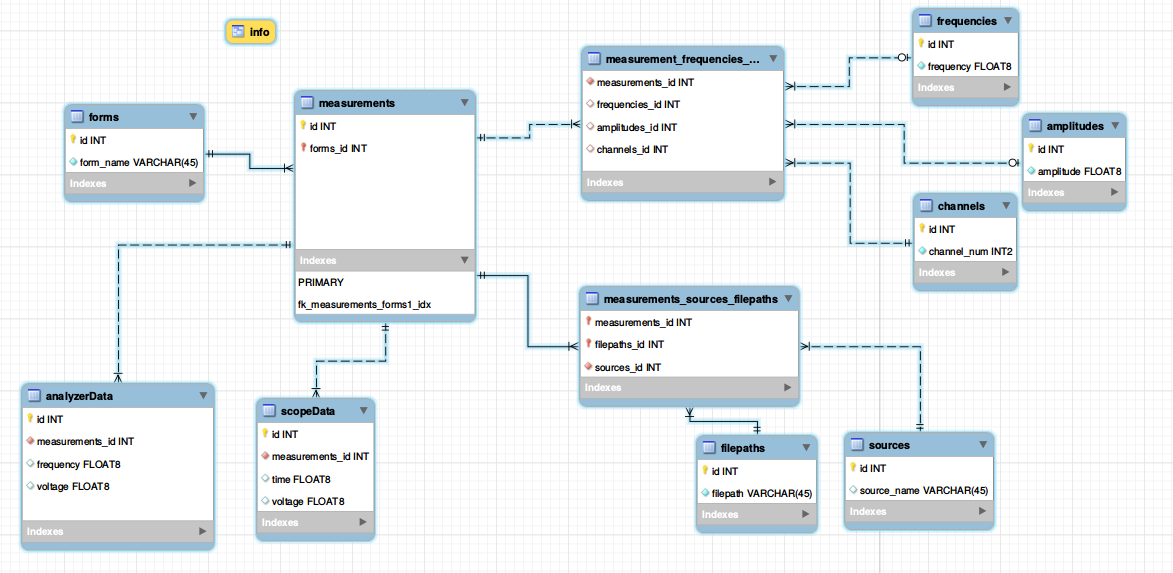
\includegraphics[width=12.5cm, height=6cm]{figures/figure1.png}
        % Create a subtitle for the figure.
        \caption{EER diagram mapping the database}
        % Define the label of the figure. It's good to use 'fig:title', so you know that the label belongs to a figure.
        \label{fig:fig1}
\end{tcolorbox}
\end{minipage}
\end{figure}

The little yellow box entitled ``Info" corresponds to a view, or saved query
that allows for easier access to the desired data without sacrificing the
structure of an ACID database. If you were to run a simple query on the view:

\begin{figure}[H]
\centering
\begin{minipage}{.4\textwidth}
\begin{tcolorbox}
\begin{minted}{sql}
select * from info
\end{minted}
\end{tcolorbox}
\end{minipage}
\end{figure}
%\begin{verbatim}
    %SELECT * FROM info
%\end{verbatim}

You would get something back that looks like:
\begin{figure}[H]
\begin{minipage}{1.12\textwidth}
\begin{tcolorbox}
    \centering
        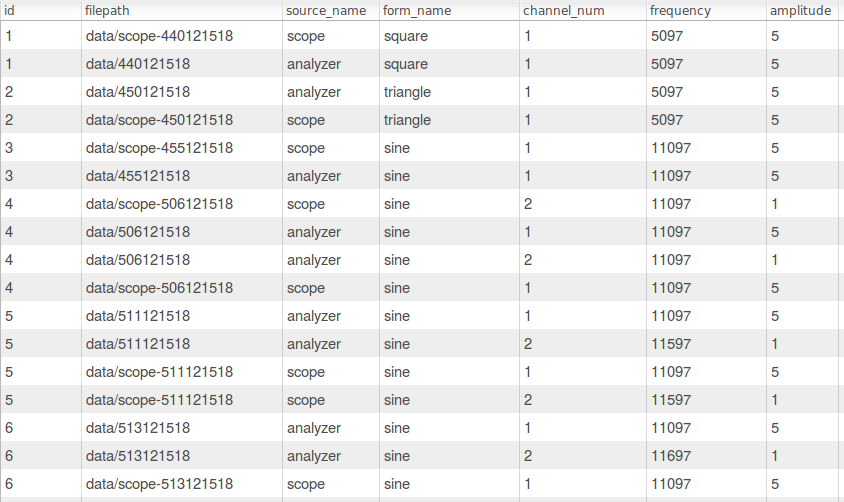
\includegraphics[width=8.9cm, height=5.3cm]{figures/figure2.png}
        \caption{A simple query on the database}
        \label{fig:fig2}
\end{tcolorbox}
\end{minipage}
\end{figure}

Hopefully all of that made sense. If not, don't worry about it -- it's not really
too relevant to the actual data analysis.
%----------------------------------------------------------------------------------------
%   SECTION 2
%----------------------------------------------------------------------------------------
\section{Objectives}

All of these labs have objectives instead of procedures. They are intended to
guide our experiments without spoon feeding us the results. Sometimes I really
miss eating bananas out of a jar. Fortunately for me, most grocery stores still
stock Gerber snacks. 

If you're not familiar with the methods and procedures of this lab, then I
would suggest reviewing the manual. It is quite extensive and details all the
theory far more eloquently than I ever could. It lives in:

\begin{figure}[H]
\centering
\begin{minipage}{.8\textwidth}
\begin{tcolorbox}
\begin{minted}{bash}
lab3/lab_descrip/Fourier_Methods_manual.pdf
\end{minted}
\end{tcolorbox}
\end{minipage}
\end{figure}

\subsection{Introduction to Spectrum Analyzers}

\subsubsection{Sine, Square, and Triangle Waves}%
\label{ssub:sine_square_and_triangle_waves}

The first thing we did in lab after putting our heads on straight was run a few
single frequency waves through the oscilloscope and spectrum analyzer. The goal
of this section was to get comfortable with the conversion between frequency
and time domains. All of the oscilloscope data lives in the time domain.
This means that time is the independent variable and our plots consider
$Voltage(time)$. However, it is often useful and always didactic to convert
this data into $V(\omega)$ by Fourier Transforming it:

\begin{equation}
    X(\omega) = \int_{-\infty}^{\infty} x(t) e^{-i \omega t} dt
\end{equation}

Technically, we have a discreet data set that isn't quite infinite, so it might
be more accurate to say that we are using a Fourier Series -- but the theory is
extremely similar and a full discourse on Fourier Analysis is outside of the
scope of this report.

If we use the function generator to produce a Sine wave of 11,097 Hz, we get a
familiar looking graph of $V(t)$ on the scope:

\begin{figure}[H]
    \centering
\begin{minipage}{10cm}
\begin{tcolorbox}
        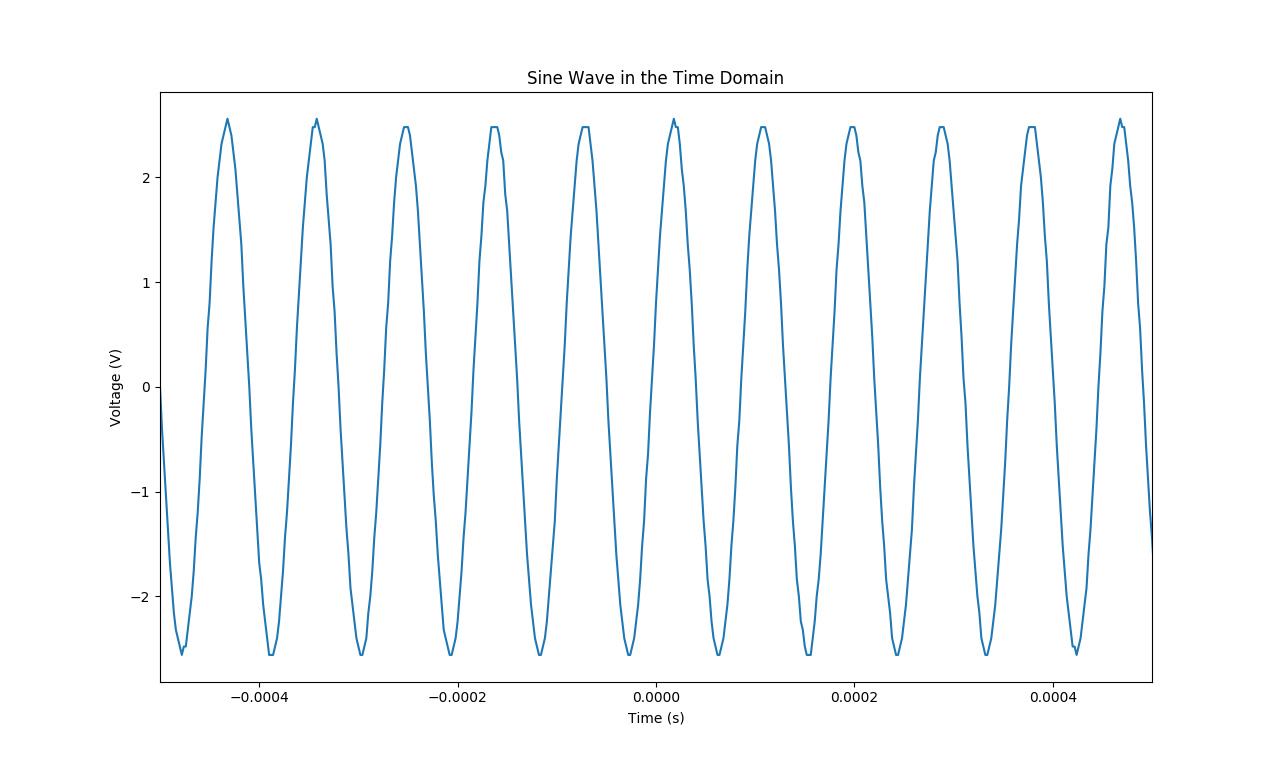
\includegraphics[width=9cm, height=5.cm]{figures/figure3.png}
        \caption{Sine wave of 11.097 kHz collected from the oscilloscope}
        \label{fig:fig3}
\end{tcolorbox}
\end{minipage}
\end{figure}

Now, everyone knows that the Fourier Transform of a sine wave is a delta
function so let's transform the data that we collected from the scope and see
how it looks:

\begin{figure}[H]
    \centering
\begin{minipage}{10cm}
\begin{tcolorbox}
        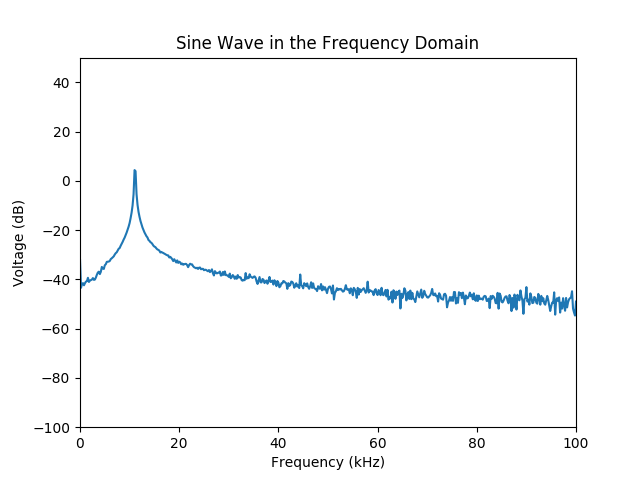
\includegraphics[width=9cm, height=6.5cm]{figures/figure4.png}
        \caption{FFT of data presented in Figure 3}
        \label{fig:fig4}
\end{tcolorbox}
\end{minipage}
\end{figure}

So far, it seems like all is well in the world, but let's overlay the results
with the data collected from the SR770 and see whether things actually match
up.

\begin{figure}[H]
    \centering
\begin{minipage}{11cm}
\begin{tcolorbox}
        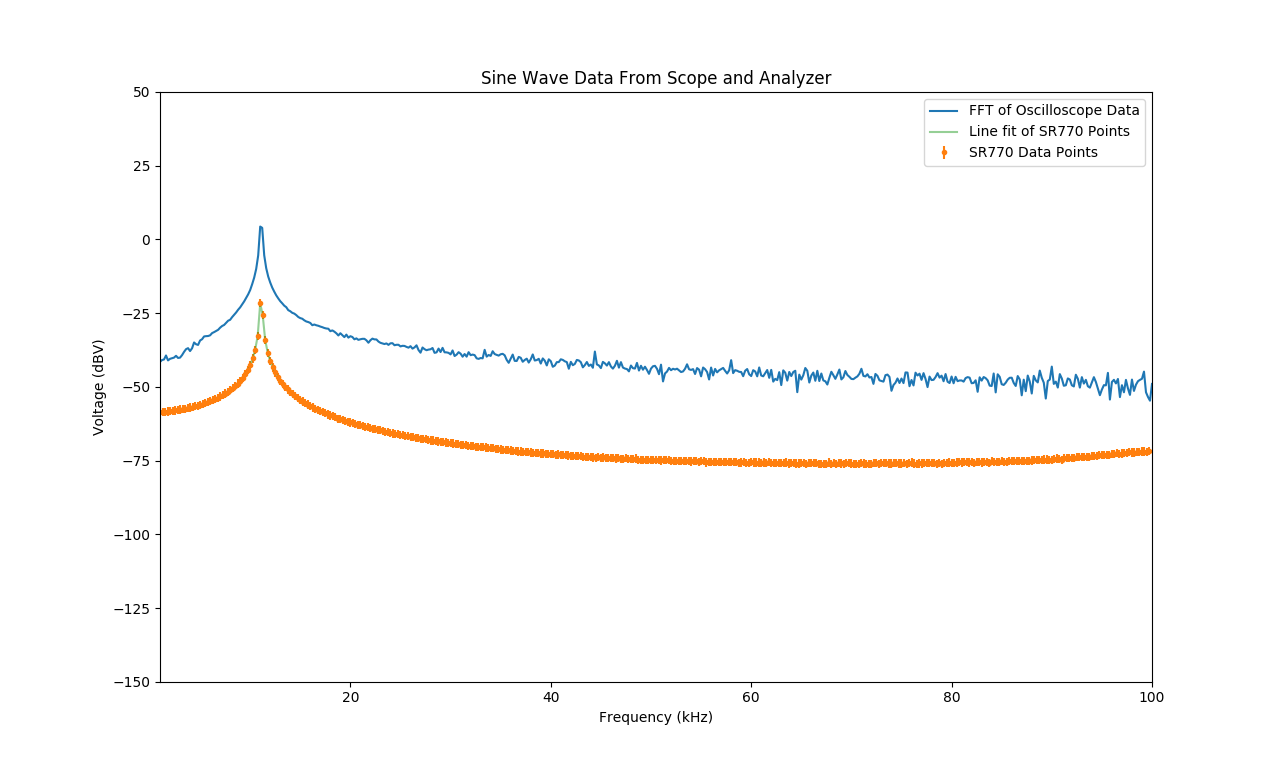
\includegraphics[width=10cm, height=6.cm]{figures/figure5.png}
        \caption{Analyzer data overlaid on top of Figure 4}
        \label{fig:fig5}
\end{tcolorbox}
\end{minipage}
\end{figure}

Things are looking pretty good -- however, those amplitudes don't quite seem to
match. At a glance that might seem problematic. But, if you look closer at the
label on my y-axis, you'll notice that the units are not the same! The data
from the SR770 is in dBV while the data from the oscilloscope is in dB. In
fact, if you convert everything to a linear scale, multiply by the amplitude of
the input current, and convert back to a log scale -- the amplitudes just about
match up:

\begin{figure}[H]
    \centering
\begin{minipage}{11cm}
\begin{tcolorbox}
        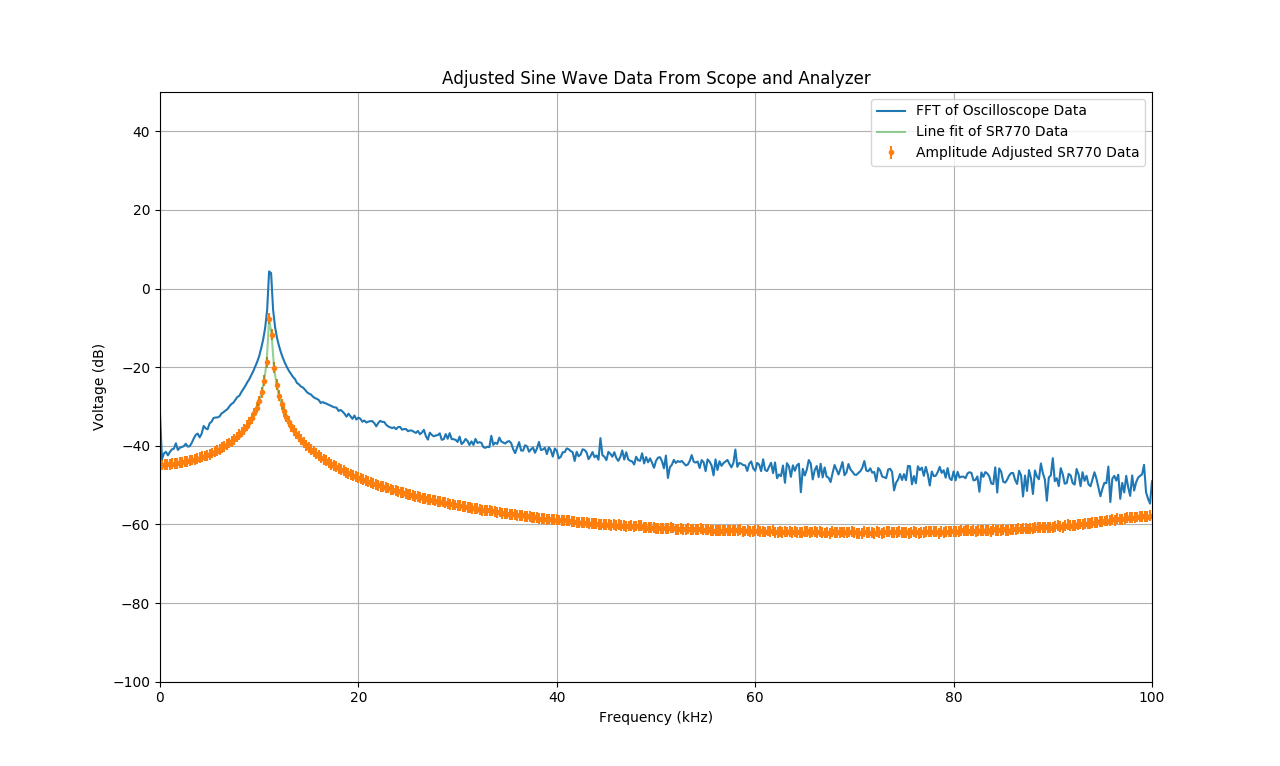
\includegraphics[width=10cm, height=6.cm]{figures/figure6.png}
        \caption{Amplitude matching by converting dBV to dB}
        \label{fig:fig6}
\end{tcolorbox}
\end{minipage}
\end{figure}

The last thing to do before moving on is model the results. The plot is
starting to get a little bit loud, but modeling a sine wave is quite easy. All
we have to do is plug in the frequency, transform a vector of points, and
overlay the final plot in the series
\begin{figure}[H]
    \centering
\begin{minipage}{11cm}
\begin{tcolorbox}
        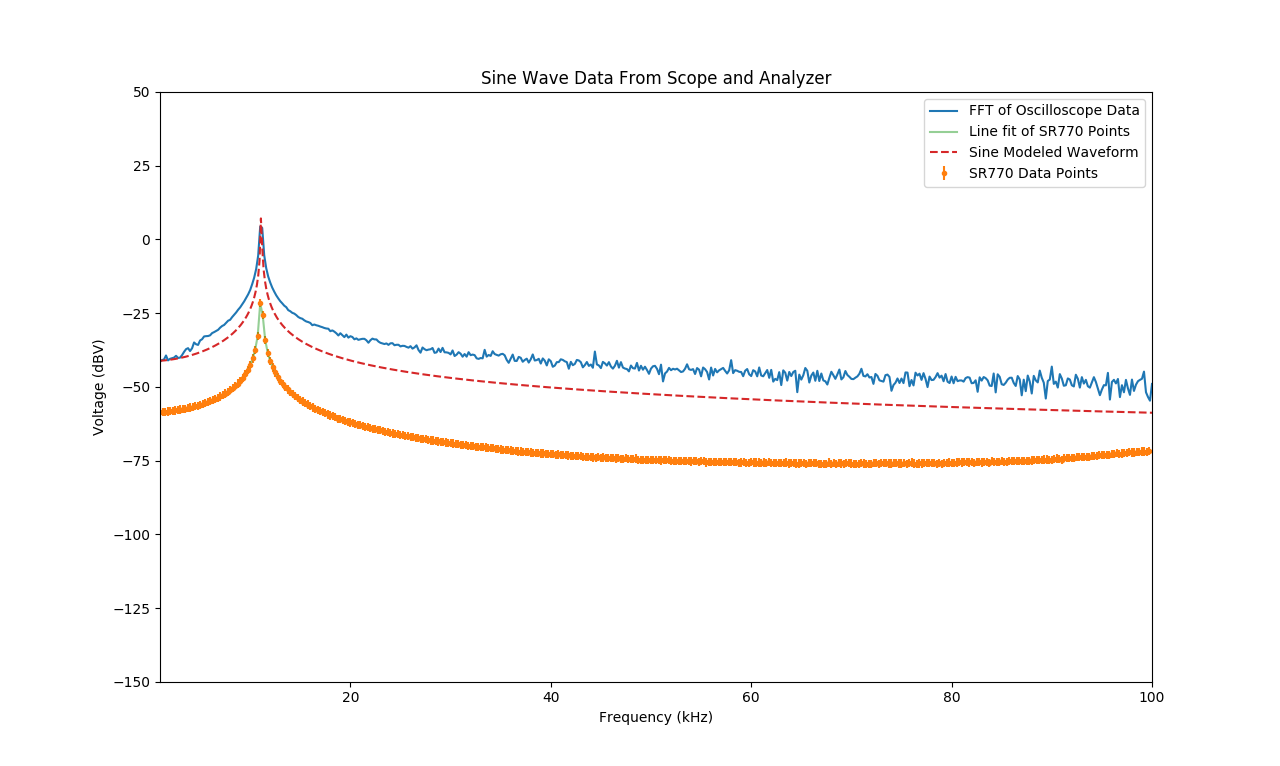
\includegraphics[width=10cm, height=6cm]{figures/figure7.png}
        \caption{Integrating a theoretical model to Figure 6}
        \label{fig:fig7}
\end{tcolorbox}
\end{minipage}
\end{figure}

The coding aspect of this lab was extensive enough that it seemed
to warrant utilizing classes. So, I defined a class for measurements. The
attributes for this class could be a useful reference, so here they are: 

\begin{figure}[H]
\centering
\begin{minipage}{1\textwidth}
\begin{tcolorbox}
\begin{verbatim}
    :measurementId: Int - unique identifier 

    :an: Pandas DF - holds all analyzer data

    :xan: Pandas DF - uncertainties and values in x
    :yan: Pandas DF - uncertainties and values in y

    :xanvalues: Pandas DF - values for x component
    :yanvalues: Pandas DF - values for y component

    :xanerror: Pandas DF - uncertainties for x component
    :yanerror: Pandas DF - uncertainties for y component

    :sc: Pandas DF - holds all oscilloscope data

    :xsc: Pandas DF - holds values for x component
    :ysc: Pandas DF - holds values for y component
\end{verbatim}
\end{tcolorbox}
\end{minipage}
\end{figure}

I can't say that I'm especially proud of the class method for taking a Fourier
Transform, but it does get the job done. 

This method is available to any instances of the measurement class:
\begin{figure}[H]
\centering
\begin{minipage}{1\textwidth}
\begin{tcolorbox}
\begin{minted}{python}
    def fourierTransformVoltage(self):
        """
        :returns: nothing - however, will fourier transform, 
        normalize, convert voltage to dB, and set all the 
        necessary variables for plotting
        """

        try:
            #pick out values and time step
            self.voltage = self.voltage.apply(lambda x: x.n)
            self.time = self.time.apply(lambda x: x.n)

            #perform the transformation on voltage
            fftvolt = np.fft.fft(self.voltage)

            #clean up and normalize
            fftvolt = np.fft.fftshift(fftvolt)
            fftvolt= 2*fftvolt/float(len(self.voltage))

            #convert voltage to dB
            self.fftdbv = 20.*np.log10(np.abs(fftvolt))

            #determine the time step and window length
            self.time_step = self.time[2]- self.time[1]
            self.win_length = len(self.time)

            #recover frequency bins
            self.fftfreq = np.fft.fftfreq(
                self.win_length, self.time_step)

            self.fftfreq = np.fft.fftshift(self.fftfreq)

            #convert to kHz
            self.fftfreq = self.fftfreq/1000.

            self.xsc = self.fftfreq
            self.ysc = self.fftdbv

        #all code to contine if fft fails
        except Exception as e:
            print('could not perform FT: ', e)
\end{minted}
\end{tcolorbox}
\end{minipage}
\end{figure}




The data that we collected is available in data/magnetic.xlsx 
and my lab notebook, so I will not recopy it here. But, here is what it looks
like:

\begin{figure}[H]
        % Center the figure.
        \begin{center}
        % Include the eps file, scale it such that it's width equals the column width. You can also put width=8cm for example...
        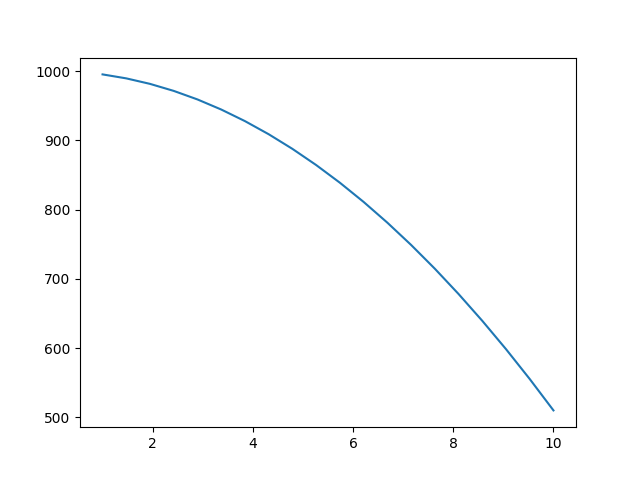
\includegraphics[width=8cm, height=6cm]{/home/johnny/kod/py/bin/venv/py3/phx444/labs/lab2/figures/figure1.png}
        % Create a subtitle for the figure.
        \caption{Plotting the Measured values for Magnetic Field}
        % Define the label of the figure. It's good to use `fig:title', so you know that the label belongs to a figure.
        \label{fig:fig_1}
        \end{center}
\end{figure}
I chose to read my data into python as a Pandas DataFrame. In my experience,
pandas is just about the best library to work with heterogeneous data. It's
even able to read an excel file:
\begin{center}
\begin{minipage}[t]{.75\textwidth}
\begin{lstlisting}[frame=tlrb]
xl = pd.ExcelFile(`data/magnetic.xlsx')
df = xl.parse(`Sheet1')
\end{lstlisting}
\end{minipage}
\end{center}
After that, I dropped the non-existent entries off the bottom of the DataFrame
because they're problematic for model fitting. Then, I used the uncerainties
package and a lambda function to propagate error through all of our mass and 
current measurements. I'm not going to copy all of the code here, but the
general syntax follows this form:
\begin{center}
\begin{minipage}[t]{.75\textwidth}
\begin{lstlisting}[frame=tlrb]
<Measurement>= \
    df[<Measurement>].dropna().apply(
        lambda x: ufloat(x, <error>)
    )
\end{lstlisting}
\end{minipage}
\end{center}
Next, for the current menasurements, I looked up the specs for
Keithley's model 2000 6 1/2 digit multimeter. I stared at them for a while.
Then I pestered Brian for a while. Then I stared at the specs some more. Eventually, I
pestered Brian enough that he showed how to read the table. In our case, the current 
has an uncertainty of:
$$(1000 \times I + 3 \times 15) \times 10^{-6}$$
In python, we are able to make use of the pandas data structure and
uncertainties library to propagate this:
\begin{verbatim}
current_error = \
    1000 * df[`current'].dropna() * 10 ** -6 + 3 * 15 * 10**-6

b_cal_current = \
    pd.Series(uarray(df[`current'].dropna(), current_error))
\end{verbatim}
Notice that I have to explicitly turn the result back into a
pandas object. The uarray() method returns a NumPy Array. It would be totally
fine to leave the result as a NumPy object, but syntactically NumPy is slightly
different and Pandas, so it's beneficial to have all objects be the same type.

I was able to fit the curve using the same method as in the data
analysis lab. Specifically, I assumed linearity and fit it with:

\begin{center}
\begin{minipage}[t]{.75\textwidth}
\begin{lstlisting}[frame=tlrb]
def lin_fit(x, a, b):
    return a*x + b

popt, pcov = curve_fit(
                lin_fit, 
                current_values, 
                b_cal_values
            )

b_fit = lin_fit(
    current_values, 
    *popt
)
\end{lstlisting}
\end{minipage}
\end{center}

We learned last lab that residuals are a pretty decent sanity check on the
accuracy of data and models. So let's go ahead and plot the residuals from this
fit:

\begin{center}
\begin{minipage}[t]{.75\textwidth}
\begin{lstlisting}[frame=tlrb]
r_i = b_cal_values - b_fit

plt.errorbar(
    current_values,
    r_i,
    yerr=b_cal_error,
    fmt='o')
\end{lstlisting}
\end{minipage}
\end{center}

And showing this plot, we find that the residuals are actually quite
reasonable. They are clustered around zero and their error bars are easily
visible. Notice that the size of the error bars around zero is quite large.
This makes sense because the current error ought to be similar in magnitude, but
its fractional error will increase:

\begin{figure}[H]
        % Center the figure.
        \begin{center}
        % Include the eps file, scale it such that it's width equals the column width. You can also put width=8cm for example...
        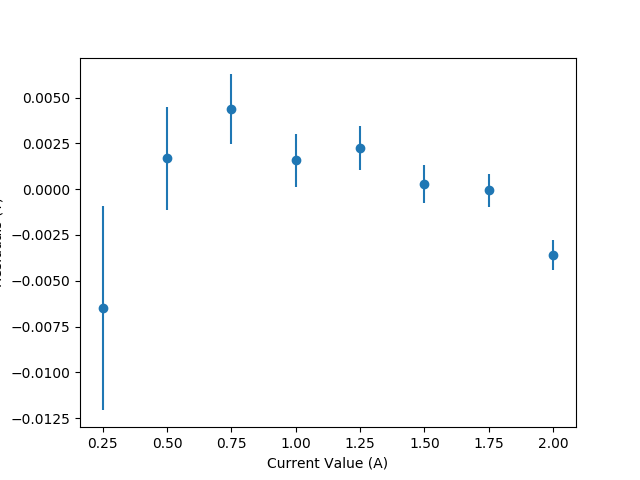
\includegraphics[width=8cm,
        height=6cm]{/home/johnny/kod/py/bin/venv/py3/phx444/labs/lab2/figures/figure1b.png}
        % Create a subtitle for the figure.
        \caption{Plotting the residuals as a sanity check}
        % Define the label of the figure. It's good to use `fig:title', so you know that the label belongs to a figure.
        \label{fig:fig_2}
        \end{center}
\end{figure}


\subsection{Magnetic Susceptibility of Samples}
Now, hopefully I've convinced you that the environment between our magnets
houses a magnetic field that is approximately .4 Teslas. If I haven't
convinced you yet, try this:

\begin{center}
\begin{minipage}[t]{.75\textwidth}
\begin{lstlisting}[frame=tlrb]
def understand(paper, confused=True):
    if confused:
        read(section_1)
        read(section_2)
        understand(paper)

    return 
\end{lstlisting}
\end{minipage}
\end{center}

Moving right along, We massed all our samples using the Guoy balance. Then, we
did some math to determine how much of our sample was empty space and how much
was really the substance in question. For example, if you have a vial full of pebbles, then
a good bit of the vial is actually just air. The actual area is given by:
$$A = (w\times l)(\% real)$$
Where \% real is: 
$$\frac{ m_{measured}}{ m_{theoretical}}$$
And, for a substance of known density $\rho$, theoretical mass is:
$$volume \times \rho$$
Putting all of that together with the equation that we derived in lecture, we
find the magnetic susceptibilty with:
$$\chi_m = \frac{2 \times \mu_0 \times g (m_1 - m_0)}{A B^2}$$
As before, $m_1$ refers to the mass of the magnet apparatus with the sample
sitting in between the magnet and $m_0$ is the mass of the magnet without a
sample in between it. 

One peculiarity that I had not considered prior to doing my data analysis was
the possibility of getting a value larger than 1 for \% real. This does not
physically make sense (because our samples were not pressurized). For most of the
samples, this was not an issue. 

However, for the two wire samples, things got a little
interesting. The wires were too small for us to measure very accurately which
led us to accumulate immensely large errors.  After thinking on the issue for a
while, eventually I decided to accept the measurements on these wires that are
provided in the lab to be exact. I also decided to refuse negatve percentages
and cap the maximum \% real at 1. 

In python, we can impose reaonability on percentages with: 

\begin{center}
\begin{minipage}[t]{.75\textwidth}
\begin{lstlisting}[frame=tlrb]
percent_real = (real_mass / theory_mass)

percent_real.apply(
    lambda x: ufloat(min(abs(x.n), 1), x.s)
)
\end{lstlisting}
\end{minipage}
\end{center}

Then, we can drop the error from cobalt:

\begin{center}
\begin{minipage}[t]{.75\textwidth}
\begin{lstlisting}[frame=tlrb]
area[4] = area[4].n
percent_real[4] = percent_real[4].n
\end{lstlisting}
\end{minipage}
\end{center}

And now we're off to the races! Doing all the math things and putting them in a
table thing that compares measurements and uncertainties to accepted $\chi_m$
values, we see that most of our results are actually quite good:

\begin{figure}[H]
        % Center the figure.
        \begin{center}
        % Include the eps file, scale it such that it's width equals the column width. You can also put width=8cm for example...
        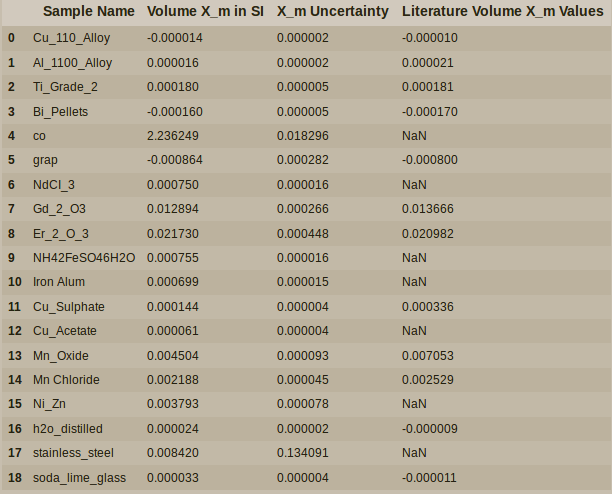
\includegraphics[width=10cm, height=10cm]{/home/johnny/kod/py/bin/venv/py3/phx444/labs/lab2/figures/tablefigure.png}
        % Create a subtitle for the figure.
        \caption{A table with our results}
        % Define the label of the figure. It's good to use 'fig:title', so you know that the label belongs to a figure.
        \label{fig:fig_4}
        \end{center}
\end{figure}

However, there were a couple of surprises! I was shocked at the lack
of literature data for comparison. Most of the data that I \textit{was} able to
find was not available in SI units. The conversion from $\chi_{molar}$ in cgs
to volume $\chi_m$ in SI must be done in 2 steps. First, you convert to volume
$\chi_m$ in cgs and second, you multiply by the conversion factor of $4 \pi$.
These units are very picky and I still don't fully understand why.

Also, it seems as though something went a bit wrong when we prepared our own
samples! While the majority of our data falls within 3 $\sigma$ of the
literature values, we did not even get the correct sign for Water or Soda Lime
Glass. Maybe we should have been a bit more suspicious of the bottle labeled
``distilled water."



%----------------------------------------------------------------------------------------
%   SECTION 4
%----------------------------------------------------------------------------------------
\section{Questions}
\subsection{Units Of $\chi_m$}

There are a few common units for $\chi_m$ because there are a few different
flavors of susceptibility. In class we discussed that Volume $\chi_m$ is
actually unitless. This is true in both cgs and SI - however, there \textit{is
    still a conversion factor between them}. I find that pretty strange, but I
learned to stop questioning units when I started measuring the mass of the sun
in kilometers.

You might also encounter a molar $\chi_m$. In CGS this has units of
$\frac{cm^3}{mol}$ but Brian told us that in SI, molar $\chi_m$ has units of
$\frac{kg}{mol}$. That's pretty neat, but Wikipedia disagrees with Brian.
Wikipedia says that molar $\chi_m$ has units of $\frac{m^3}{mol}$ in SI.

The last type of $\chi_m$ that Brian mentioned is mass $\chi_m$. In SI this has
units of $\frac{m^3}{kg}$ while in cgs it is $\frac{cm^3}{g}$.

\subsection{Compare Results to Literature Values}
It's tough to compare our results to literature values, because quite a few of
the literature values don't exist. And, when they do exist they're in the wrong
units. So, in order to do any comparison I had to start by collecting as many
literature values for $\chi_m$ as I could find. I converted the cgs values of
$\chi_{mol}$ into volume $\chi_m$ in SI like this:
$$\chi_{sivol} = 4 \pi\frac{\chi_{cgsmol}}{M_{cgs} / \rho_{cgs}} $$
Where M is the molar mass. If we plot this with the literature values along the
x axis and measure values along the y axis, we would expect the line y = x to
intersect most of them. I went one step further and ran a linear fit on our
data points using the same curve\_fit method that I describe in section 2.1.
Plotting the results, we see that, overall, our data agrees with the
literature:


\begin{figure}[H]
        % Center the figure.
        \begin{center}
        % Include the eps file, scale it such that it's width equals the column width. You can also put width=8cm for example...
        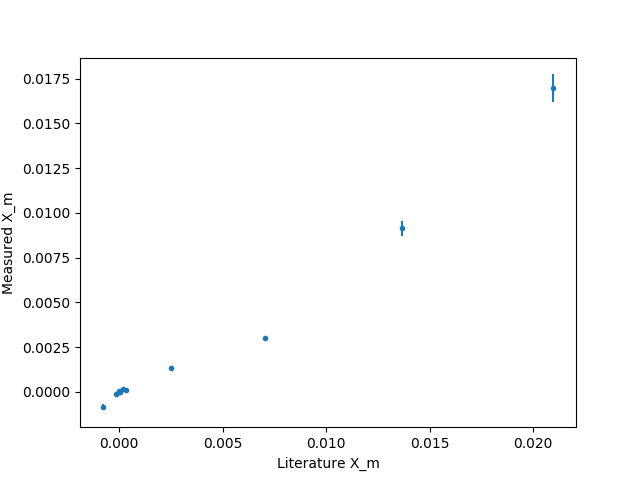
\includegraphics[width=8cm, height=6cm]{/home/johnny/kod/py/bin/venv/py3/phx444/labs/lab2/figures/figure8.png}
        % Create a subtitle for the figure.
        \caption{Plotting accepted values for $\chi_m$ against our measurements}
        % Define the label of the figure. It's good to use 'fig:title', so you know that the label belongs to a figure.
        \label{fig:fig_5}
        \end{center}
\end{figure}

\subsection{Levitation!!}
Brian gave this one away. I'm going to go out on a limb here and say that
pyrolitic graphite might work, just maybe. Here's what it looks like:


\begin{figure}[H]
        % Center the figure.
        \begin{center}
        % Include the eps file, scale it such that it's width equals the column width. You can also put width=8cm for example...
        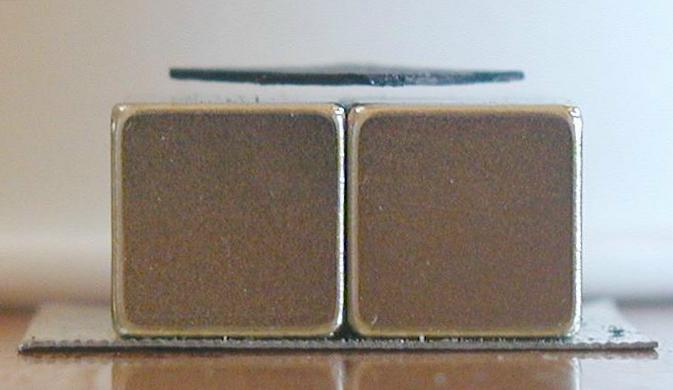
\includegraphics[width=8cm, height=6cm]{/home/johnny/kod/py/bin/venv/py3/phx444/labs/lab2/figures/levitation.jpg}
        % Create a subtitle for the figure.
        \caption{Photo credits to the kind folks over at: http://sci-toys.com}
        % Define the label of the figure. It's good to use 'fig:title', so you know that the label belongs to a figure.
        \label{fig:fig_6}
        \end{center}
\end{figure}

Sci-toys has a really great explanation of the phenomenon. It's worth reading
if you like science. Here's an excerpt that will (hopefully) get you excited
enough to open up a browser:
\begin{quotation}

 ``We can do that by using four magnets. The poles of the magnets push on the
 diamagnetic material more strongly than other parts of the magnet. With four
 magnets, the four edges of the square of pyrolytic graphite will be pushed
 away from the four poles."

 - sci-toys.com

\end{quotation}

\section{Conclusion and Sources of Error}

I must say, I'm pretty impressed with our results. I fully expected them to
wildly disagree with the accepted values of $\chi_m$. During the experiment, we
noticed that the instruments were incredibly sensitive. Things like leaning on
the table, or rotating the balance made noticeable impacts upon results. We
also noticed that the scale's calibration had a tendency to walk. And, paralax
made it quite difficult to ensure that the bottom of our samples was precisely
in the middle of the magnetic field. 

The only significant source of error seemed to occur during the preparation of
our own samples. It's possible that the vials were not adequately cleaned. It's
even possible that the samples we prepared were not quite exactly what we
thought they were. Lastly, it's possible that the literature values for
$\chi_m$ are wrong.

If I were to do this experiment again, I would be more careful to monitor the
walking of the scale's calibration and more careful while preparing my own
samples.

\end{document}
